\stopallthesefloats
\section{Benchmark Implementation}
\label{sec:identification:implementation}
This section explains how the strategy presented in
Section~\ref{sec:identification:strategy} has been implemented on the NXP QorIQ
T4240 architecture.

\subsection{The NXP QorIQ T4240}
\begin{figure}[hbt!]
\begin{center}
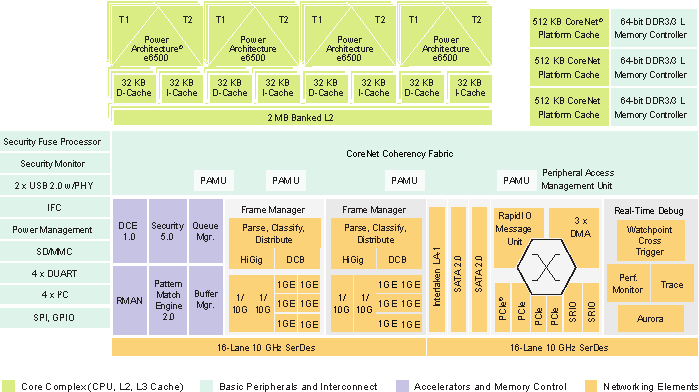
\includegraphics[width=\textwidth]{\chapterdirectory/figure/full_t4240.pdf}
\end{center}
\caption{Architecture Block Diagram (Figure taken from \cite{T4240})}%
\label{fig:full_t4240}
\end{figure}

Figure~\ref{fig:full_t4240} gives an overview of the NXP QorIQ T4240
architecture, a PowerPC featuring twelve e6500 cores, each of which is capable
of running two simultaneous threads. The cores are equally distributed among
three clusters, with one shared 2MB L2 cache per cluster. These three L2 caches
coordinate and access memory through a complex interconnect called the CoreNet
Coherency Fabric. According to their processor's documentation, \cite{e6500},
these clusters implement the MESI cache coherence protocol. The architecture's
documentation, \cite{T4240} indicates that the caches are able to perform
\textit{cache intervention} (caches may provide a data reply if they hold the
relevant memory element).

\begin{figure}[hbt!]
\begin{center}
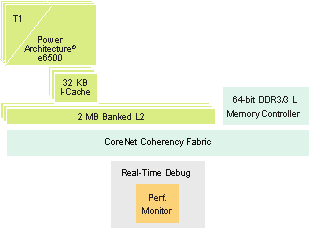
\includegraphics[width=0.6\textwidth]{\chapterdirectory/figure/minimal_t4240.pdf}
\end{center}
\caption{Components used in the Identification Process}
\label{fig:t4240_experimental_setup}
\end{figure}

In order to limit the mechanisms observed to the L2 cache coherence, the
architecture's L1 Data caches were deactivated during this process. Furthermore,
only a single core (and execution thread) per cluster (and thus, per L2 cache)
was considered. In an attempt at reducing the impact of instruction fetching,
the L1 Instruction caches stayed enabled. Lastly, the system only used a single
memory controller. Thus, the resulting configuration resembled the one shown in
Figure~\ref{fig:t4240_experimental_setup}, the remaining hardware configuration
having been left to what it is by default.

\begin{limitation}[No Observation Available from the Coherence Manager]
\label{lim:no_cmgr}
The coherence manager, if one is present, cannot be observed directly through
the available means.
\end{limitation}

\subsection{Naught}
To perform the benchmarks, a small bare-metal library was created:
\textit{Naught}\footnote{\url{https://github.com/nsensfel/naught}}. It
simplifies access to the architecture's performance monitors by providing C
functions equivalent to those used in the algorithm of
Figure~\ref{fig:micro_bench:co_running_apps_cots_algo_part_one}.  Naught offers
a very crude implementation of barriers, making it possible to synchronize the
code running on each core. It also has a similarly crude implementation of
semaphores, ensuring that any output made by the software does not end up
garbled.

After some testing, the architecture's monitors were found to be slightly
imprecise: even with all monitors of a core being set to track the same
activities,
they would yield slightly different results (staying generally within a
difference of 10 recorded occurrences). In order to address this issue, and to
reduce the impact of the extra activities performed by Naught's code logic
(loop iterator increase, for example), the benchmarks are applied over a set
of 8000 memory elements.

All cores access these same 8000 memory elements. Each memory element has a size
corresponding to that of a cache line, and is properly aligned so as to be fully
stored within one (i.e.~no false sharing is occurring, see
Appendix~\ref{app:false_sharing}).

\begin{figure}[hbt!]
\begin{center}
\begin{tabular}{c}
\begin{lstlisting}
SrcStates = [STATE_A, STATE_B, STATE_C];
reach_states(core_id, SrcStates);
start_monitors();
SysInstruction = [INSTR_A, INSTR_B, INSTR_C];
perform(instructions[core_id]);
join(barrier);
store_monitor_results();
\end{lstlisting}
\end{tabular}
\end{center}
\caption{Implementation of the \benchmark{} function}
\label{fig:identifying:benchmark_implementation}
\end{figure}

The benchmark being run on the architecture corresponds to an implementation of
the \benchmark{} function (see
Definition~\ref{def:identifying:benchmark_function}), and is executed by all
cores of the architecture in parallel. In effect, this corresponds to a single
iteration of the inner loop from
Figure~\ref{fig:identification:state_exploration}.
Figure~\ref{fig:identifying:benchmark_implementation} provides an overview of
the \benchmark{} implementation.

\begin{figure}[hbt!]
\begin{center}
\begin{tikzpicture}[->,>=stealth',shorten >=1pt,auto,node distance=4cm,
                    semithick]
   \node[initial,state] (S0)                 {\lstinline![I, I, I]!};
   \node[state]         (S1) [right of=S0]   {\lstinline!SrcStates!};
   \node[state]         (S2) [right of=S1]   {\lstinline![?, ?, ?]!};

   \path
      (S0) edge node { \lstinline!reach_state! } (S1)
      (S1) edge node { \lstinline!perform! } (S2)
   ;
\end{tikzpicture}
\end{center}
\caption{Evolution of caches coherence states}
\label{fig:identifying:cache_state_evol}
\end{figure}

The architecture starts in its initial state (\emph{init}), and must thus reach
the \lstinline!SrcStates! prior to the instructions being executed (see
Figure~\ref{fig:identifying:cache_state_evol}). This is done by
\lstinline!reach_states! and explained in
Section~\ref{sec:identification:initializing_caches}. Once the caches have
reached the relevant states, the \lstinline!start_monitors! function enables the
performance monitors, as detailed in
Section~\ref{sec:identifying:perf_monitors}. The relevant instructions
(\lstinline!SysInstruction!) can then be executed. The chosen assembly
instructions are explained in
Section~\ref{sec:identifying:performing_instructions}. A barrier is used to
ensure all cores have completed their instructions before results are reported.
\lstinline!store_monitor_results! is explained in
Section~\ref{sec:identifying:data_recording}, and is how the performance
monitors and resulting system state are retrieved by the user.

\subsection{Initializing the Caches (Lines 1 \& 2 of
Figure~\ref{fig:identifying:benchmark_implementation})}
\label{sec:identification:initializing_caches}
\lstinline!SrcStates! indicates, for each of the three caches, the stable
coherence state that the memory element must be in before the measures start.
There are two possible cases:
\begin{itemize}
\item
   The \lstinline!SrcStates! is \lstinline![INVALID, INVALID, INVALID]!,
   and nothing needs to be done.
\item
   \lstinline!SrcStates! was previously reached somehow, and a sequence of
   instructions for each core leading to it is thus known and was added to
   the \lstinline!reach_states! function.
\end{itemize}

In effect, the \lstinline!reach_states! function follows similar idea to the one
from Section~\ref{sec:nehalem}: the different cores cannot simply reach their
target state by themselves, and must thus be coordinated.

The \lstinline!reach_states! initially does nothing, and instructions are added
as new system states are reached so that they may be reached again from the
\emph{init} (\lstinline![INVALID, INVALID, INVALID]!) state. Let us now consider
the \lstinline!reach_states! function as it is defined after the application
of the identification process on the T4240 has completed.

\begin{figure}[hbt!]
\begin{center}
\begin{tabular}{c}
\begin{lstlisting}
operation_a();
join(barrier_a);
operation_b();
join(barrier_b);
operation_c();
join(barrier_c);
\end{lstlisting}
\end{tabular}
\end{center}
\caption{Overview of the \lstinline!reach_states! function}
\label{fig:identifying:reach_states_fun}
\end{figure}

Figure~\ref{fig:identifying:reach_states_fun} provides an overview of the
\lstinline!reach_states! function. This function is performed by each core,
but the \lstinline!operation_a()!, \lstinline!operation_b()!,
\lstinline!operation_c()! are defined depending on both the executing core's
target \lstinline!SrcStates! and its left neighbor's.

At the end of the identification process, the \lstinline!reach_states! function
was defined with to the following rules. If the core has to:
\begin{itemize}
\item \textbf{Reach Modified:}
   \lstinline!operation_a()! writes the memory elements, the other operations do
   nothing.
\item \textbf{Reach Exclusive:}
   \lstinline!operation_a()! reads the memory elements, the other operations do
   nothing.
\item \textbf{Reach Shared:}
   \lstinline!operation_a()! reads the memory elements, the other operations do
   nothing.
\item \textbf{Reach Forward:}
   \lstinline!operation_a()! and the others do nothing, but
   \lstinline!operation_b()! reads the memory elements.
\item \textbf{Reach Invalid:}
   Given the state of the cache on the left (computed using
   \lstinline!modulo(core_id - 1, 3)!):
   \begin{itemize}
      \item \textbf{Modified:} nothing is done.
      \item \textbf{Exclusive:} nothing is done.
      \item \textbf{Shared:} \lstinline!operation_b()! reads the memory elements
         and \lstinline!operation_c()! empties the cache.
      \item \textbf{Forward:} \lstinline!operation_a()! reads the memory
         elements and \lstinline!operation_c()! empties the cache.
      \item \textbf{Invalid:} nothing is done.
   \end{itemize}
\end{itemize}

\subsection{Enabling the Performance Monitors (Line 3 of Figure~\ref{fig:identifying:benchmark_implementation})}
\label{sec:identifying:perf_monitors}
\begin{property}[T4240 Performance Counters]
\label{pro:t4240:performance_counters}
Below is a list of the monitorable activities of interest, as well as their
meaning based on what I understand them to be.
\begin{itemize}
\item \textbf{L2 Data Accesses} Accesses made to the L2 cache.
\item \textbf{L2 Snoop Hits}
   External queries on a memory element held by this cache.
\item \textbf{L2 Snoop Pushes} Replies given to snooped queries.
\item \textbf{External Snoop Requests} External queries.
\item \textbf{L2 Reloads From CoreNet} Replies received.
\item \textbf{L2 Snoops Causing MINT}
   Replies to a snooped query when holding the memory element in a
   \textit{dirty} (modified) state.
\item \textbf{L2 Snoops Causing SINT}
   Replies to a snooped query when holding the memory element in a
   \textit{clean} (unmodified) state.
\item \textbf{CPU Cycles}
\end{itemize}
\end{property}

The \lstinline!start_monitors()! operation configures each of the available
performance counters of the core to track the occurrence of different
monitorable
activities
(see Property~\ref{pro:t4240:performance_counters}), then resets their value and
activates them. Unlike with the papers in Chapter~\ref{cha:micro-benchs}, all
cores record the activities, not just a single one. Since there are 8 different
activities to monitor and each core has four performance monitors, two runs of
each benchmark is necessary in order to capture all the relevant information.

\subsection{Performing Instructions (Lines 4 \& 5 of
Figure~\ref{fig:identifying:benchmark_implementation})}
\label{sec:identifying:performing_instructions}
The \lstinline!perform(instructions[core_id])! call will perform either
\loadinstr{}, \storeinstr{}, or \evictinstr{} on each of the 8000 memory
elements, depending on which instruction was set for \lstinline!core_id! in the
\lstinline!SysInstruction! array.

The NXP QorIQ T4240 architecture does not feature the \evictinstr{}
instruction. The closest available instruction (\texttt{dcbi}, \textit{Data
Cache Block Invalidate}) results in the element being evicted from all the
caches, which is significantly different, unless that element has been marked as
ignored by cache coherence (which is then pointless for the purposes of cache
coherence identification). Since the benchmarks employed here are very small
programs dealing almost exclusively with the set of experimental memory
elements, the application of an  \evictinstr{} on all of the memory elements was
replaced by a simple invalidation of the whole local cache, which still does
involve cache coherence.

The \storeinstr{} is implemented using \textit{stw} (\textit{Store Word}), which
writes a zero to the memory element.

The \loadinstr{} is implemented using \textit{lwz} (\textit{Load Word and
Zero}), which writes a reads the memory element's value and stores it into an
otherwise unused register.

\subsection{Data Recording (Lines 6 \& 7 of
Figure~\ref{fig:identifying:benchmark_implementation})}
\label{sec:identifying:data_recording}
Once every core has completed their operations and \lstinline!join(barrier)!,
the \lstinline!store_monitor_results()! prints the number of recorded values
for each type of monitorable activity on each core. This data is retrieved
through a serial connection.

\begin{property}[T4240 Observable Flags]
\label{pro:t4240:flags}
Cache flags can be observed using CodeWarrior, the official debugging suite for
this architecture. The observed cache line Boolean flags have the following
names: \textit{Dirty}, \textit{Valid}, \textit{Share}, \textit{Exclusive}, and
\textit{LastReader}.
\end{property}

Using CodeWarrior, the state of the caches is also recorded and stored in files,
so that the flags can be analyzed afterwards. Because the cache replacement
policy comes into play, the content of each cache is not simply that of the 8000
memory elements. Furthermore, the caches can seemingly contain multiple lines
for the same memory element, as long as at most one indicates a state other than
INVALID. The flags (see Property~\ref{pro:t4240:flags}) are easily extracted
using a simple Python script, as CodeWarrior allows exporting the content of all
caches to plain-text CSV files.

This observable information is exactly what is needed for the new entries of
both \obssystemstate{} and \archmonitorval{}.

The next section starts a description of the application of the identification
strategy on the NXP QorIQ T4240 using this benchmark implementation.

\stopallthesefloats
